\subsection{\secState{R}Cooperative Conflict Resolution}\label{sec:cooperativeConflictResolution}


\paragraph{Idea:} There is a \emph{final decision maker} (absolute authority) in conflict resolution. This authority is \emph{UTM} or \emph{air traffic attendant} with higher priority. The future \emph{UTM system} is such authority. The approach to mixed conflict resolution is mentioned in \cite{ramasamy2014towards}, based on navigation \cite{ramasamy2013novel}. This is similar to our approach. 

\begin{note}
    \emph{Open Issue:} Decentralized model with UTM as an approver of directives is possible, but that is a topic for own research.
\end{note}

\paragraph{Goal:} UAS is obligated to follow up committed mission plan with given precision.  There is one to five percent  allowed deviations for ATM mission plans.     Similar rates are achievable according to \cite{ramasamy2014towards}.  This requirement is given by \cite{icao4444} ICAO 4444 document for ATM operations.

\begin{figure}[H]
    \centering
    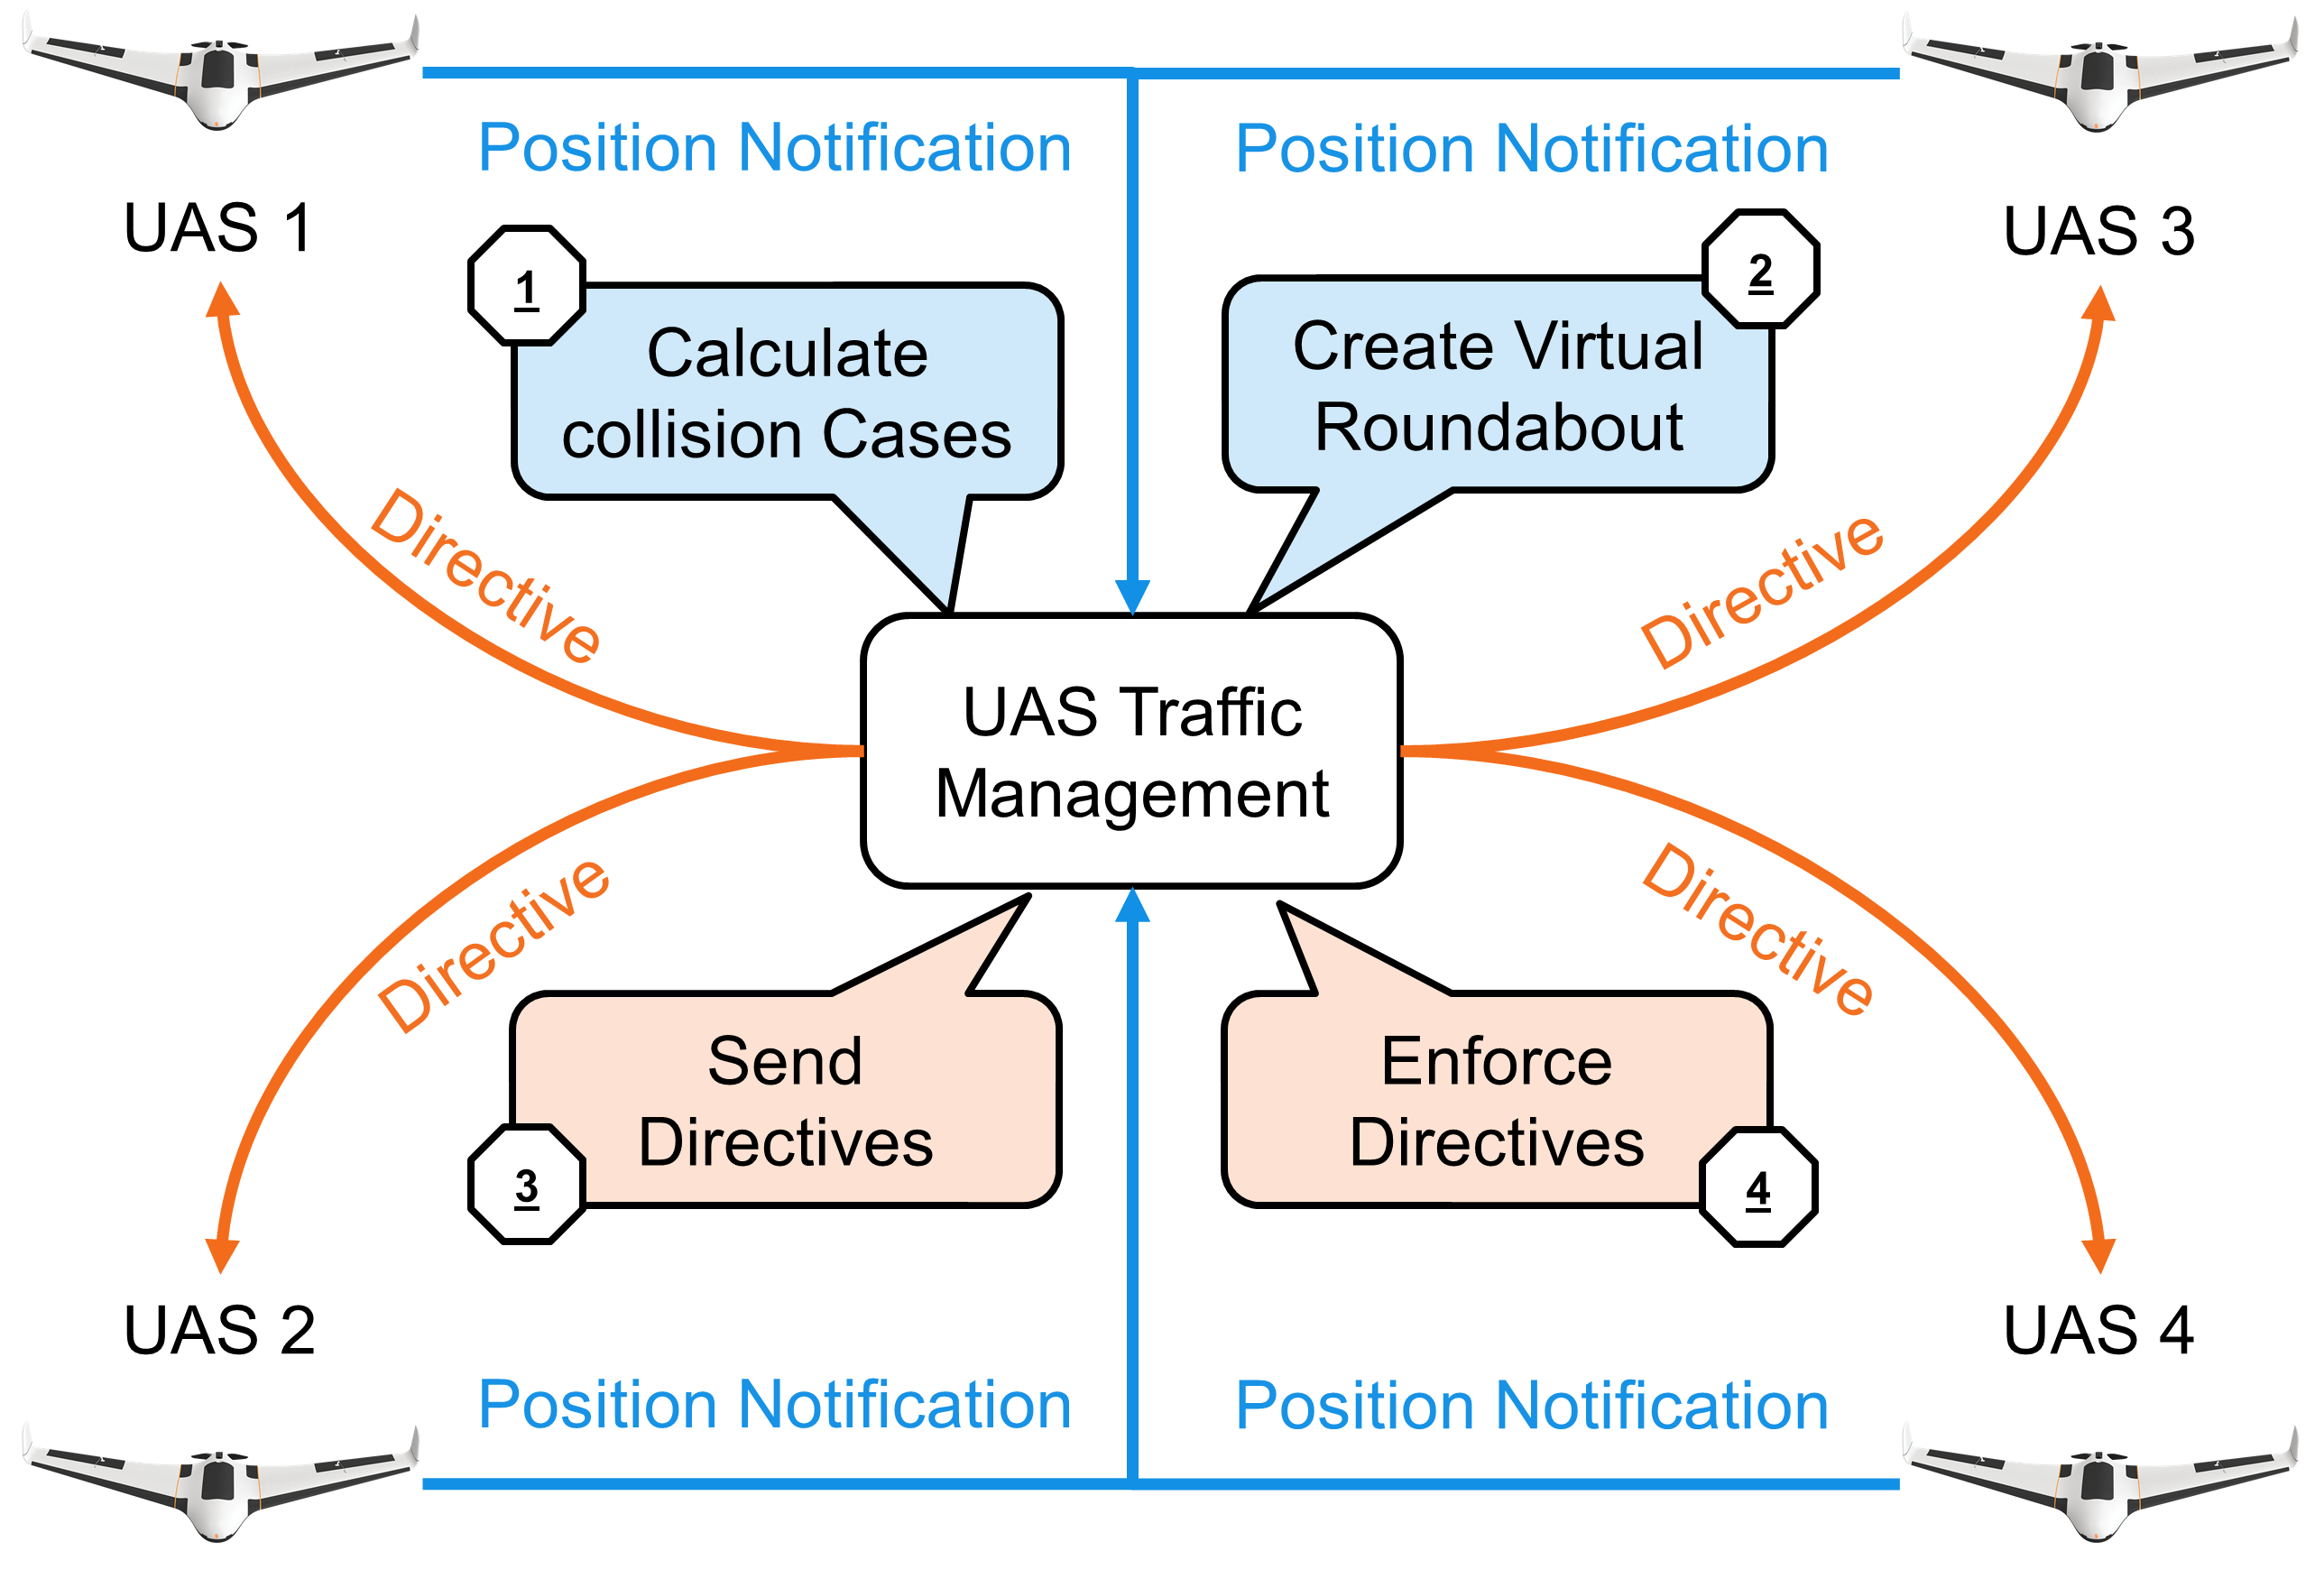
\includegraphics[width=0.7\linewidth]{\FIGDIR/RE003CooperativeResolution} 
    \caption{Cooperative conflict resolution via UTM authority.}
    \label{fig:CooperativeConflictResolutionUTM}
\end{figure}

\paragraph{Cooperative Conflict Resolution} (fig. \ref{fig:CooperativeConflictResolutionUTM}) shows a functional diagram of one \emph{UTM time-frame} there  are following actors:
\begin{enumerate}
    \item \emph{Unmanned Autonomous System} (UAS) equipped with necessary navigation and communication modules, providing the unique \emph{identification number}.
    
    \item \emph{UAS Traffic Management} (UTM) posing as the central authority for given \emph{airspace cluster}.
\end{enumerate}

\noindent The following steps are executed during \emph{Cooperative conflict resolution}:
\begin{enumerate}
    \item $UAS_* \to UTM$ \emph{Send position notification} - each \emph{UAS} is notifying the authority (UTM)
    
    \item $\circlearrowright UTM$ \emph{Calculate collision Cases} - UTM gathers data and predicts possible collisions then it tries to link them and manage the situation.
    
    \item $\circlearrowright UTM$ \emph{Create virtual Roundabout} - active collision cases are aggregated into a virtual roundabout. 
    
    \item $UTM \to UAS_*$ \emph{Send directives} - UTM sends commands to UAS systems which need to change their planned trajectories. 
    
    \item $UTM \to UAS_*$ \emph{Enforce directives} - UTM is periodically checking constraints imposed in previous \emph{decision frames}.
\end{enumerate}